%% IMPORTANT: Once working, run latex 3 times to get listoffigures to work

%% Be sure to check spelling!

%% Put **your** name and the proper due date in place

%% Copy the lstlisting and figure code as many times as you need
%% Be sure to put in your own file names if appropriate

%% Note that the \epsfig commands are currently commented out - until the
%%%% files exist, processing this code without them will result in an error
%%%% so leave the comments until you have created the graphics files!

\documentclass{article}
\usepackage{amsmath}    % loads AMS-Math package
\usepackage{epsfig}     % allows PostScript files
\usepackage{listings}   % allows lstlisting environment
\usepackage{moreverb}   % allows listinginput environment
\usepackage[letterpaper, margin=0.75in]{geometry}  % set paper size/margins

\begin{document}
\begin{center}
\rule{6.5in}{0.5mm}\\~\\
\textbf{\large EGR 103L -- Fall 2017}\\~\\
\textbf{\huge Data Analysis}\\~\\
***NAME (NetID)***\\
***Lab Section N, DAY TIMES***\\
***DATE DUE***\\~\\
{\small I understand and have adhered to all the tenets of the Duke
  Community Standard in completing every part of this assignment.  I
  understand that a violation of any part of the Standard on any part
  of this assignment can result in failure of this assignment, failure
  of this course, and/or suspension from Duke University.} 
\rule{6.5in}{0.5mm}\\
\end{center}
\tableofcontents
\listoffigures
\pagebreak

\section{Random Numbers}
Here is the diary created when the program runs:
\listinginput[1]{1}{RandDiary.txt}

\section{Hidden Images}
% discussion

\section{Chapra 2.18-2.19}
% discussion

\section{Chapra 2.22}
% discussion - use \cite[p.~51]{Chapra}

\section{Weather Data Analysis}
The specific information weather information calculated is:
\listinginput[1]{1}{WeatherDiary.txt}

\pagebreak
\appendix
\section{Codes}
% Put the name of your file in the subsection name 
% and the listinginput input
% Be sure to include the community standard in codes!

% Add \pagebreaks if they make sense

% Put the files in the same order as the problems; generally, 
% scripts will come first followed by any functions called
% by those scripts.

\subsection{GenRand.m}
\listinginput[1]{1}{GenRand.m}
\clearpage
\subsection{FindMessages.m}
\listinginput[1]{1}{FindMessages.m}
\clearpage
\subsection{RunChapra02p18.m}
\listinginput[1]{1}{RunChapra02p18.m}
\clearpage
\subsection{RunCone.m}
\listinginput[1]{1}{RunCone.m}
\clearpage
\subsection{RunWeather.m}
\listinginput[1]{1}{RunWeather.m}

\clearpage % start Figures on new page

\section{Figures}

\begin{figure}[ht!]
\begin{center}
\epsfig{file=UniformPlot.eps, width=4.5in}
\caption{Histogram of Uniformly Distributed Random Numbers.}
\end{center}
\end{figure}

\begin{figure}[ht!]
\begin{center}
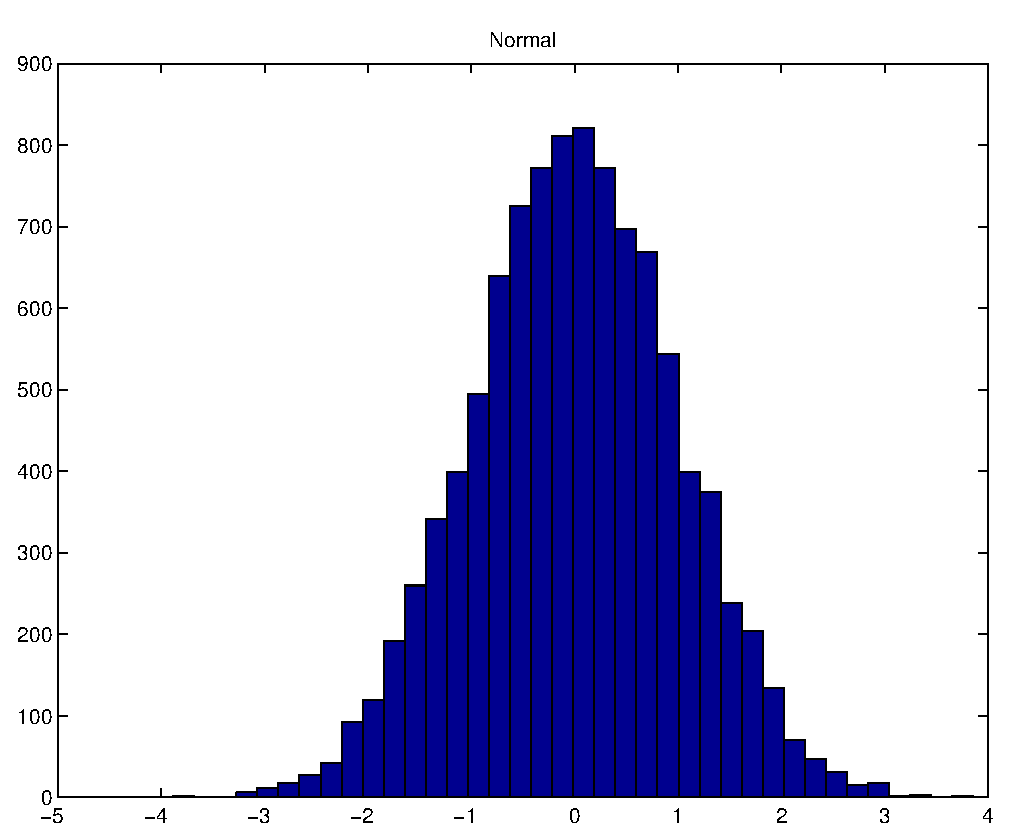
\epsfig{file=NormalPlot.eps, width=4.5in}
\caption{Histogram of Normally Distributed Random Numbers.}
\end{center}
\end{figure}

\begin{figure}[ht!]
\begin{center}
\epsfig{file=OriginalPlot.eps, width=4.5in}
\caption{Original Array.}
\end{center}
\end{figure}

\begin{figure}[ht!]
\begin{center}
\epsfig{file=GoodStartPlot.eps, width=4.5in}
\caption{First Image: ``Good Start.''}
\end{center}
\end{figure}

% Repeat the above for the rest of the images.
\clearpage

\begin{figure}[ht!]
\begin{center}
\epsfig{file=WindPlotReg.eps, width=4.5in}
\caption{Wind Tunnel Forces: Regular Plot}
\end{center}
\end{figure}

\begin{figure}[ht!]
\begin{center}
\epsfig{file=WindPlotLog.eps, width=4.5in}
\caption{Wind Tunnel Forces: Log-Log Plot}
\end{center}
\end{figure}

\begin{figure}[ht!]
\begin{center}
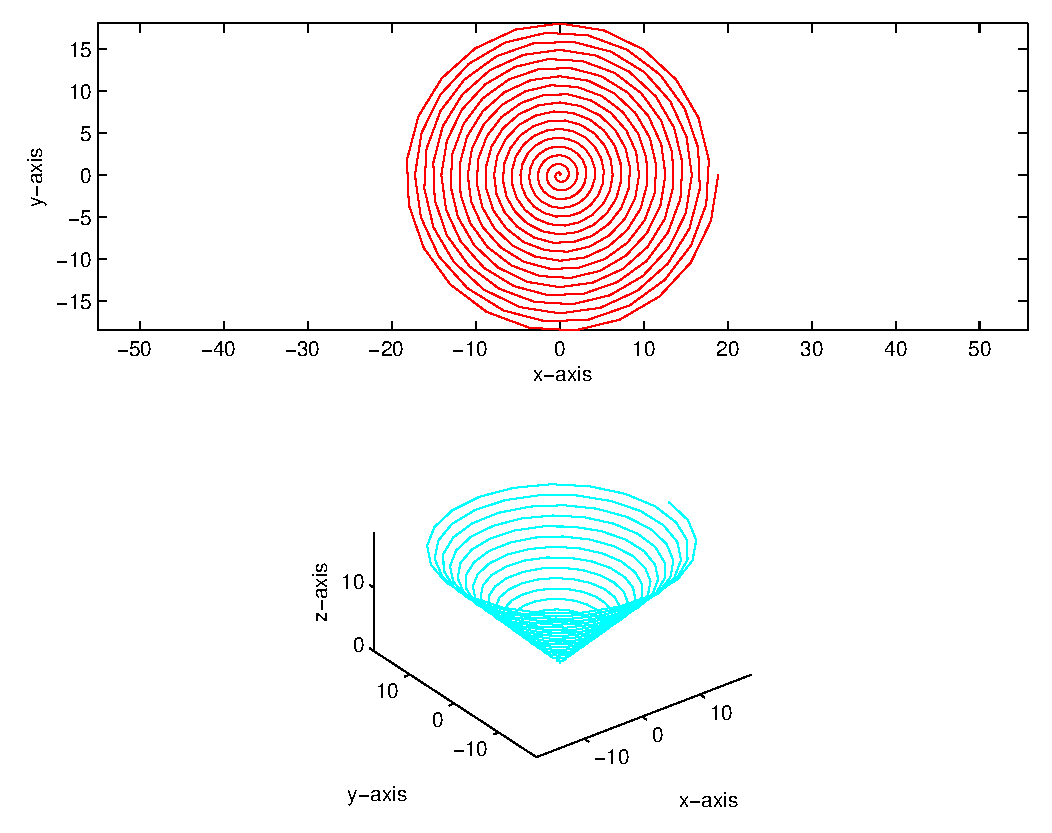
\epsfig{file=ConePlot.eps, width=4.5in}
\caption{Conical Helix Plots}
\end{center}
\end{figure}
\clearpage

\begin{figure}[ht!]
\begin{center}
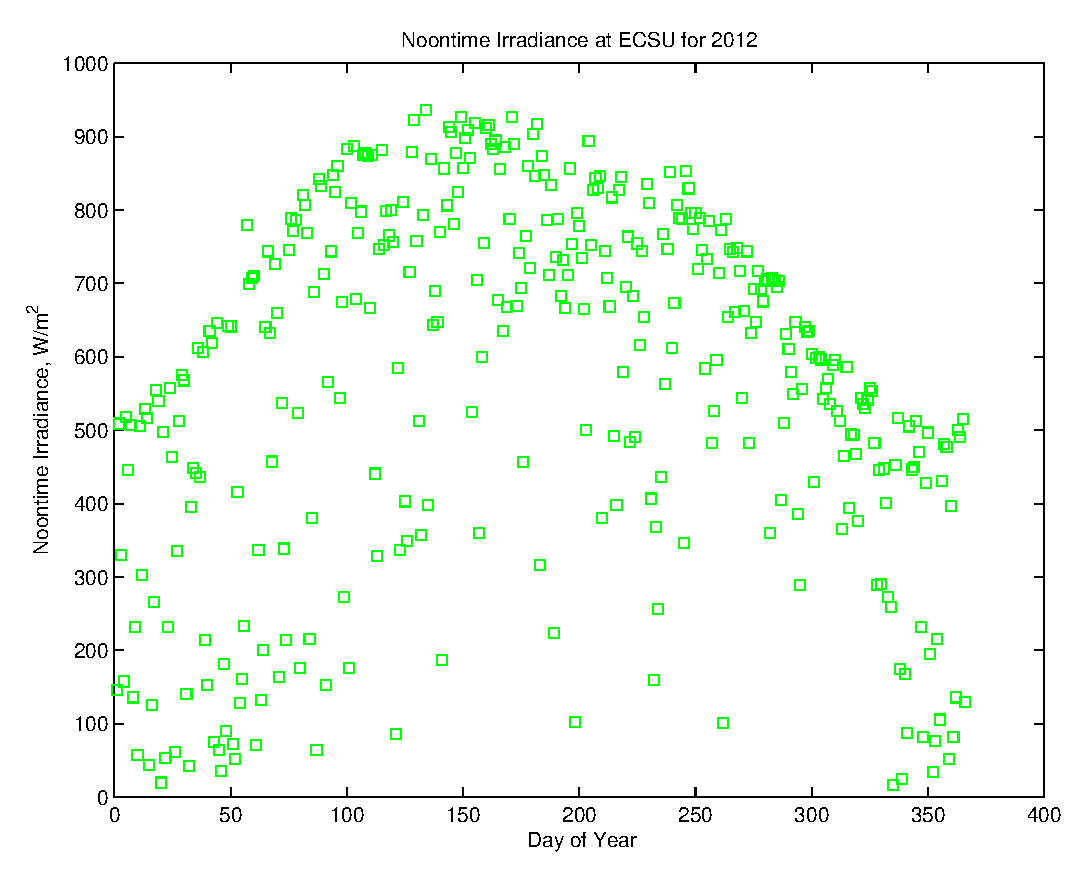
\epsfig{file=ORNLirrad.eps, width=4.5in}
\caption{Noontime Irradiance Plot}
\end{center}
\end{figure}

\begin{figure}[ht!]
\begin{center}
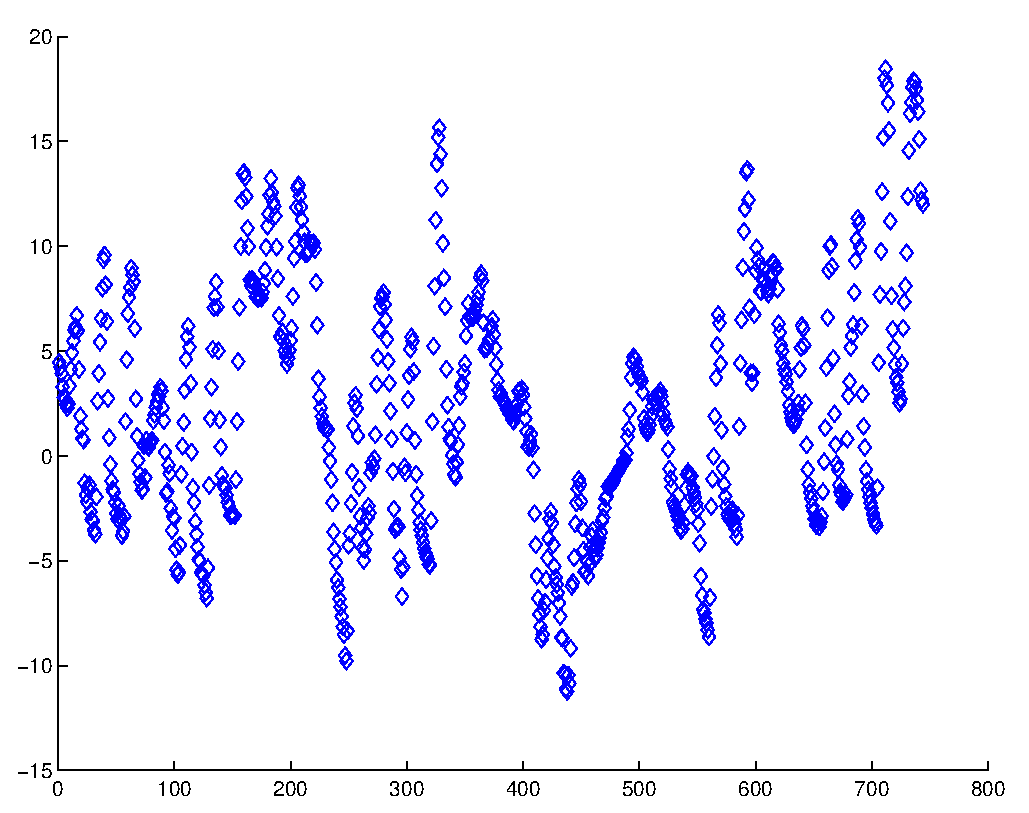
\epsfig{file=ORNLtemps.eps, width=4.5in}
\caption{January Temperatures Plot}
\end{center}
\end{figure}
\clearpage

\begin{thebibliography}{9}
\bibitem{Chapra}
  Chapra, Steven C.,
  {\it Applied Numerical Methods with MATLAB for Engineering and Scientists}.
  McGraw-Hill, New York,
  4th Edition,
  2018.
\end{thebibliography}

\end{document}

% LocalWords:  EGR 103L RandDiary txt Chapra WeatherDiary GenRand FindMessages
% LocalWords:  RunChapra02p18 RunCone RunWeather Irradiance MATLAB McGraw
